\documentclass[]{article}
\usepackage{lmodern}
\usepackage{amssymb,amsmath}
\usepackage{ifxetex,ifluatex}
\usepackage{fixltx2e} % provides \textsubscript
\ifnum 0\ifxetex 1\fi\ifluatex 1\fi=0 % if pdftex
  \usepackage[T1]{fontenc}
  \usepackage[utf8]{inputenc}
\else % if luatex or xelatex
  \ifxetex
    \usepackage{mathspec}
  \else
    \usepackage{fontspec}
  \fi
  \defaultfontfeatures{Ligatures=TeX,Scale=MatchLowercase}
\fi
% use upquote if available, for straight quotes in verbatim environments
\IfFileExists{upquote.sty}{\usepackage{upquote}}{}
% use microtype if available
\IfFileExists{microtype.sty}{%
\usepackage{microtype}
\UseMicrotypeSet[protrusion]{basicmath} % disable protrusion for tt fonts
}{}
\usepackage[margin=1in]{geometry}
\usepackage{hyperref}
\hypersetup{unicode=true,
            pdftitle={Ecological niche models of plant species exploited by Epipalaeolithic foragers in the Badia (c.~14500 BP)},
            pdfborder={0 0 0},
            breaklinks=true}
\urlstyle{same}  % don't use monospace font for urls
\usepackage{graphicx,grffile}
\makeatletter
\def\maxwidth{\ifdim\Gin@nat@width>\linewidth\linewidth\else\Gin@nat@width\fi}
\def\maxheight{\ifdim\Gin@nat@height>\textheight\textheight\else\Gin@nat@height\fi}
\makeatother
% Scale images if necessary, so that they will not overflow the page
% margins by default, and it is still possible to overwrite the defaults
% using explicit options in \includegraphics[width, height, ...]{}
\setkeys{Gin}{width=\maxwidth,height=\maxheight,keepaspectratio}
\IfFileExists{parskip.sty}{%
\usepackage{parskip}
}{% else
\setlength{\parindent}{0pt}
\setlength{\parskip}{6pt plus 2pt minus 1pt}
}
\setlength{\emergencystretch}{3em}  % prevent overfull lines
\providecommand{\tightlist}{%
  \setlength{\itemsep}{0pt}\setlength{\parskip}{0pt}}
\setcounter{secnumdepth}{0}
% Redefines (sub)paragraphs to behave more like sections
\ifx\paragraph\undefined\else
\let\oldparagraph\paragraph
\renewcommand{\paragraph}[1]{\oldparagraph{#1}\mbox{}}
\fi
\ifx\subparagraph\undefined\else
\let\oldsubparagraph\subparagraph
\renewcommand{\subparagraph}[1]{\oldsubparagraph{#1}\mbox{}}
\fi

%%% Use protect on footnotes to avoid problems with footnotes in titles
\let\rmarkdownfootnote\footnote%
\def\footnote{\protect\rmarkdownfootnote}

%%% Change title format to be more compact
\usepackage{titling}

% Create subtitle command for use in maketitle
\providecommand{\subtitle}[1]{
  \posttitle{
    \begin{center}\large#1\end{center}
    }
}

\setlength{\droptitle}{-2em}

  \title{Ecological niche models of plant species exploited by Epipalaeolithic
foragers in the \emph{Badia} (c.~14500 BP)}
    \pretitle{\vspace{\droptitle}\centering\huge}
  \posttitle{\par}
    \author{}
    \preauthor{}\postauthor{}
    \date{}
    \predate{}\postdate{}
  
\usepackage{amsmath}
\usepackage{booktabs}
\usepackage{caption}
\usepackage{longtable}

\begin{document}
\maketitle

\hypertarget{introduction}{%
\subsection{Introduction}\label{introduction}}

Species distribution models (SDM) or ecological niche models (ENM) use
data on the observed occurrences of a taxon to construct a statistical
model of its ecological niche. These models are generally then used to
predict the distribution of the species in another context, e.g.~a
region where empirical occurrence data is not available, or under past
or future climate regimes. We will attempt to model the ecological
niches of six key plant taxa for prehistoric foragers. We will use
occurrence data from Israel and Palestine, which are well-studied, to
predict the distribution of these taxa across the rest of the Southern
Levant.

First, we define our regions of interest:

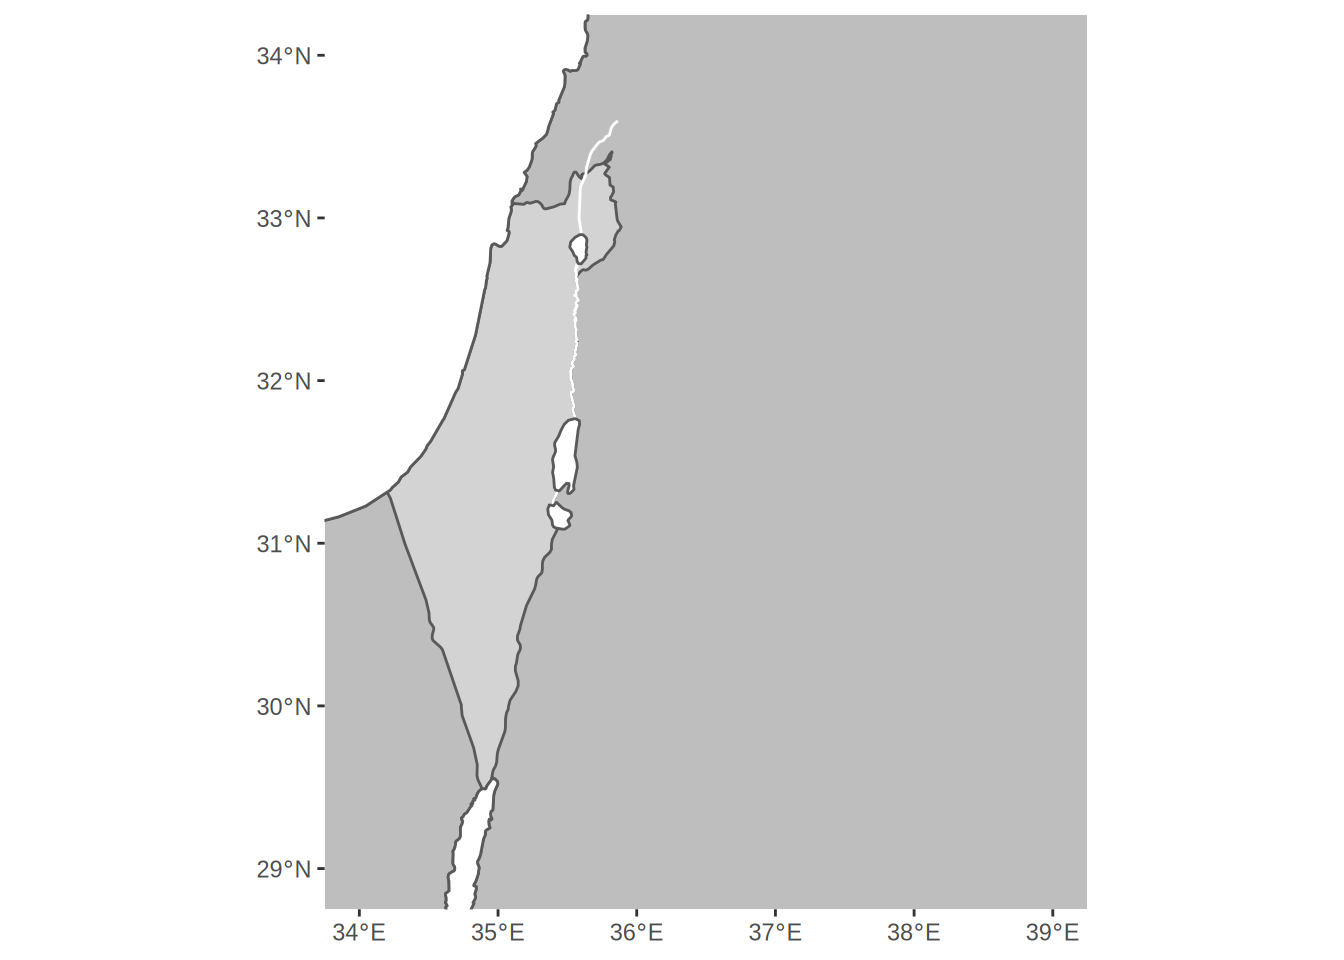
\includegraphics{analysis_files/figure-latex/regions-map-1.pdf}

\hypertarget{background}{%
\subsection{Background}\label{background}}

\hypertarget{plant-exploitation-in-the-epipalaeolithic-southern-levant}{%
\subsubsection{Plant exploitation in the Epipalaeolithic Southern
Levant}\label{plant-exploitation-in-the-epipalaeolithic-southern-levant}}

\hypertarget{ecological-niche-modelling}{%
\subsubsection{Ecological niche
modelling}\label{ecological-niche-modelling}}

\hypertarget{data}{%
\subsection{Data}\label{data}}

\hypertarget{occurrences}{%
\subsubsection{Occurrences}\label{occurrences}}

First we download species occurrence data from GBIF
(\url{https://gbif.org}). This may change, so we cache the result used
in the published analysis in \texttt{derived\_data} and only redownload
if the cached version is missing.

It's interesting to map the current distribution of these plants.
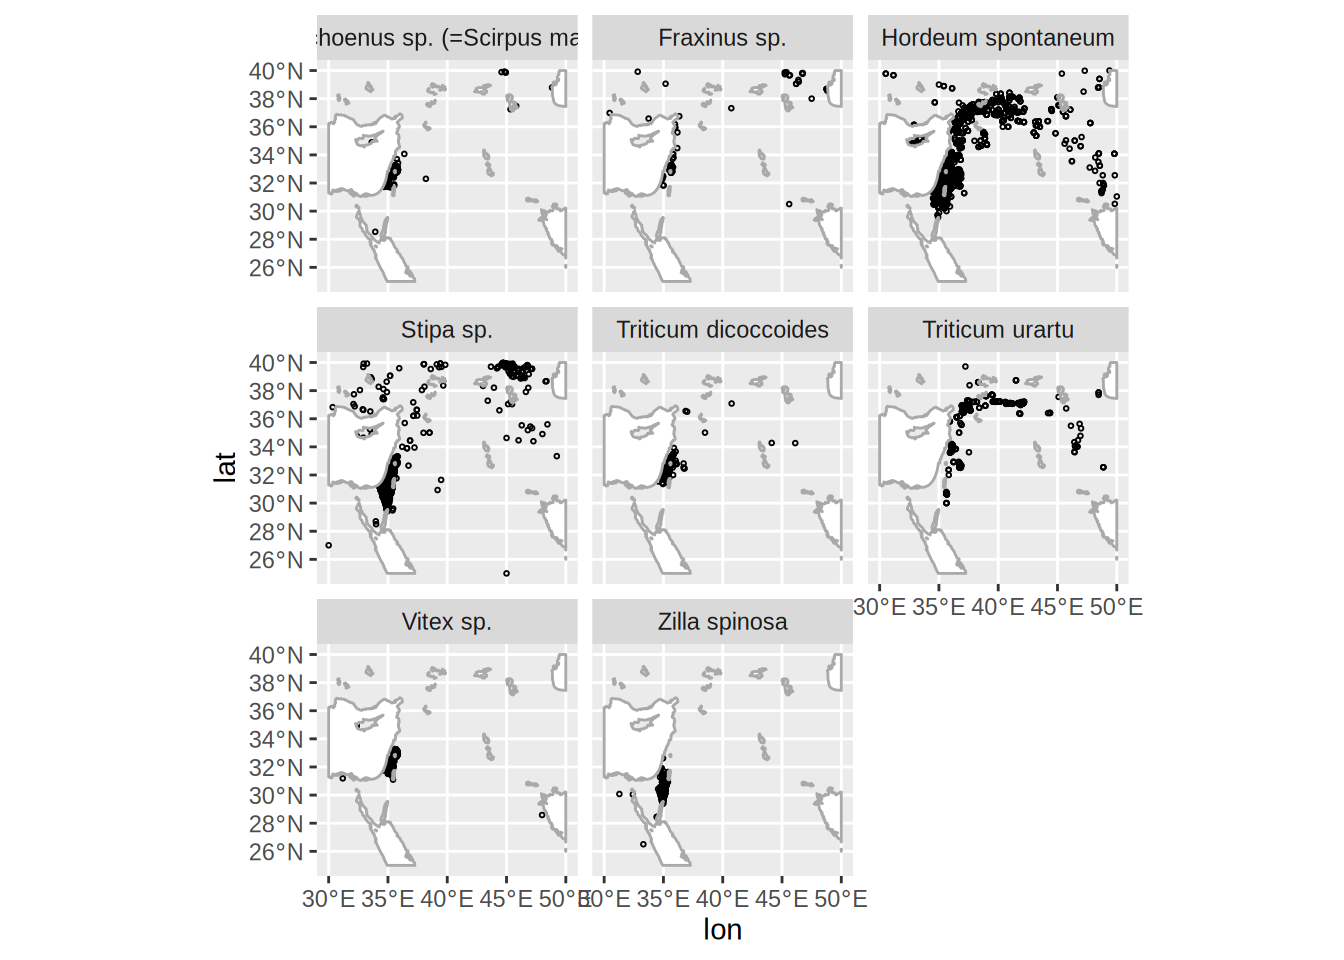
\includegraphics{analysis_files/figure-latex/occurrence-map-1.pdf}

\hypertarget{pseudo-absences}{%
\subsubsection{Pseudo-absences}\label{pseudo-absences}}

Occurrence data only tells us where a species is present; there is no
definitive information on where the species is \emph{not} found. We
therefore need to generate random background points or
``pseudo-absences'' to feed to the model. There are several ways to do
this. We follow the advice of Barbet-Massin et al.~(2012) for
regression-based species distribution models and use a large
(\textasciitilde10000) random sample of points, weighted equally against
the presences in the regression.

\hypertarget{environmental-data}{%
\subsubsection{Environmental data}\label{environmental-data}}

\hypertarget{current-climate}{%
\paragraph{Current climate}\label{current-climate}}

To construct the model, we'll use a standard set of ``bioclimatic''
predicator variables. These sixteen variables are derived from monthly
precipitation and temperate data:

\captionsetup[table]{labelformat=empty,skip=1pt}
\begin{longtable}{lll}
\toprule
biovar & definition & formula \\ 
\midrule
bio1 & Mean annual temperature &  \\ 
bio2 & Mean diurnal range &  \\ 
bio3 & Isothermality & (bio2 / bio7) * 100 \\ 
bio4 & Temperature seasonality & sd(temp) * 100 \\ 
bio5 & Maximum temperature of warmest month &  \\ 
bio6 & Minimum temperature of coldest month &  \\ 
bio7 & Annual temperature range & bio5 - bio6 \\ 
bio8 & Mean temperature of wettest quarter &  \\ 
bio9 & Mean temperature of driest quarter &  \\ 
bio10 & Mean temperature of warmest quarter &  \\ 
bio11 & Mean temperature of coldest quarter &  \\ 
bio12 & Total annual precipitation &  \\ 
bio13 & Precipitation of wettest month &  \\ 
bio14 & Precipitation of driest month &  \\ 
bio15 & Precipitation seasonality &  \\ 
bio16 & Precipitation of wettest quarter &  \\ 
bio17 & Precipitation of driest quarter &  \\ 
bio18 & Precipitation of warmest quarter &  \\ 
bio19 & Precipitation of coldest quarter &  \\ 
\bottomrule
\end{longtable}

Here the current bioclimatic data is from CHELSA
(\url{http://chelsa-climate.org/bioclim/}).

\hypertarget{palaeoclimate}{%
\paragraph{Palaeoclimate}\label{palaeoclimate}}

\hypertarget{soil}{%
\subsubsection{Soil}\label{soil}}

Velazco et al.~(2017) have shown that edaphic data, recently available
on a global scale, is usefully combined with bioclimatic data in
modelling plant niches.

We use data from SoilGrids, a global map of soil characteristics derived
from remote sensing classification at 1km resolution.

\hypertarget{terrain}{%
\subsubsection{Terrain}\label{terrain}}

There are also relevent aspects of the terrain that can be easily
derived from a digital elevation model. We'll use NASA-JPL's SRTM v3 3
arc-second resolution DEM, smoothed with Sun's denoising algorithm
{[}TODO: CITE{]}. Slope was calculated from this surface using GDAL
3.0.0 and the topographic wetness index (TWI) using the r.topidx module
of GRASS 7.8. The DEM was reprojected to a conformal projection (Jordan
Transverse Mercator, EPSG:19995) for these calculations, using a
bilinear interpolation, then back to geographic coordinates.

\hypertarget{model}{%
\subsection{Model}\label{model}}

\hypertarget{selection-of-predictors}{%
\subsubsection{Selection of predictors}\label{selection-of-predictors}}

We reviewed existing floras to identify specific variables from these
datasets that are relevant to the niche of our target taxa. The results
are summarised below.

\begin{verbatim}
## Parsed with column specification:
## cols(
##   Taxon = col_character(),
##   Factor = col_character(),
##   Notes = col_character(),
##   Reference = col_logical()
## )
\end{verbatim}

\captionsetup[table]{labelformat=empty,skip=1pt}
\begin{longtable}{llc}
\toprule
Factor & Notes & Reference \\ 
\midrule
\multicolumn{1}{l}{Triticum sp.} \\ 
\midrule
Precipitation & Adapted to dry conditions, at least 400 mm per annum for T. dicoccoides, or 300–350 mm for T. urartu and T. boeoticum. & NA \\ 
Soil type & T. urartu and T. boeoticum prefer basalt calcareous soils. & NA \\ 
Soil acidity & Found in acidic soils (limited distribution) & NA \\ 
Terrain & 100 m asl to 1600–1650 m asl. T. dicoccoides grows on mountain slopes. & NA \\ 
\midrule
\multicolumn{1}{l}{Hordeum spontaneum} \\ 
\midrule
Precipitation & Adapted to dry conditions, at least 200–250 mm rainfall per annum. & NA \\ 
Temperature & Not tolerant of cool conditions. & NA \\ 
Soil type & Tolerant of poor calcareous soils. & NA \\ 
Terrain & Grows on rocky limestone slopes, marly banks, and waste places, between 30 and 1650 m asl. & NA \\ 
\midrule
\multicolumn{1}{l}{Stipa sp.} \\ 
\midrule
Terrain & Grows on limestone mountain slopes between 400 and 2500 m asl. & NA \\ 
\midrule
\multicolumn{1}{l}{Vitex sp.} \\ 
\midrule
Water & Grows close to water resources, banks of streams and dry wadis & NA \\ 
Terrain & No higher than 750 m asl, mostly on sandy groumd, alluvial soils, rocky areas, dry river beds. & NA \\ 
\midrule
\multicolumn{1}{l}{Zilla spinosa} \\ 
\midrule
Soil type & Sandy deserts, dry soils, stony ground. & NA \\ 
\midrule
\multicolumn{1}{l}{Bolboschoenus glaucus} \\ 
\midrule
Water & A wetland plant, it grows in the shores of the lakes, often underwater. The subspecies maritimus (sea club-rush) grows in freshwater or saline marshes with Typha, Juncus and Phragmites, stagnant swamps, water meadows with Orchis palustris, by streams and rivers, dried up river beds, soda lakes, thermal springs, saline and alluvial flats, beaches, edge o/irrigation ditches and rice fields. & NA \\ 
Salinity & Some club rush like sea-club-rush can tolerate high salinity. & NA \\ 
Terrain & Grows anywhere between 0 and 2000 m asl. & NA \\ 
\midrule
\multicolumn{1}{l}{Fraxinus sp.} \\ 
\midrule
Water & Along with rivers and streams. 400-1900 small, by streams often in comparatively dry and rocky places & NA \\ 
Terrain & Mostly dryish, rocky places, in macchie, deciduous scrub or forest, Pinus brutia or P. nigra forests, or mixed forest, 650–1700 m asl. & NA \\ 
\bottomrule
\end{longtable}

Based on these results, we made the following initial selection of
predictor variables to build the models.

\captionsetup[table]{labelformat=empty,skip=1pt}
\begin{longtable}{llll}
\toprule
Variable & Units & Dataset & Source code \\ 
\midrule
\multicolumn{1}{l}{Climate} \\ 
\midrule
Minimum temperature of coldest month & °C ×10 & PaleoClim 1.0 & bio\_6 \\ 
Total annual precipitation & mm & PaleoClim 1.0 & bio\_12 \\ 
Precipitation of wettest month & mm & PaleoClim 1.0 & bio\_13 \\ 
Precipitation of driest month & mm & PaleoClim 1.0 & bio\_14 \\ 
Precipitation seasonality & σ/μ & PaleoClim 1.0 & bio\_15 \\ 
\midrule
\multicolumn{1}{l}{Soil} \\ 
\midrule
Organic carbon content & g per kg fine earth & SoilGrids250m & ORCDRC\_M\_sl2\_250m \\ 
Coarse fragment content & \% volume & SoilGrids250m & CRFVOL\_M\_sl2\_250m \\ 
Sand content & \% mass & SoilGrids250m & SNDPPT\_M\_sl2\_250m \\ 
Acidity & pH ×10 in H2O & SoilGrids250m & PHIHOX\_M\_sl2\_250m \\ 
Depth to bedrock & cm (up to 200 cm) & SoilGrids250m & BDRICM\_M\_250m \\ 
\midrule
\multicolumn{1}{l}{Terrain} \\ 
\midrule
Elevation & m & SRTM DEM v3 & srtm1v3s\_slevant \\ 
Slope & ° & SRTM DEM v3 & srtm1v3s\_slevant\_slope \\ 
Topographic Wetness Index & ln(upslope area / tan(slope)) & SRTM DEM v3 & srtm1v3s\_slevant\_twi \\ 
\bottomrule
\end{longtable}

One aspect that we cannot easily incorporate into the models is the
interaction between these taxa and other plant and animal species:
cereal grasses grow best when they have no competition from perennial
plants, \emph{Fraxinus} often grows in scrub or forest, and so on.

We also lack data for soil salinity so far.

These datasets come with different resolutions. To use them all in the
same analysis, we resample them all to the finest dataset (the SRTM
terrain variables, at 3 arc-second resolution).

We will model the ecological niche of each species using a generalised
linear regression.

First we extract the values of the predictor variables at each
occurrence and pseudo-absence location:

\hypertarget{species-response-curves}{%
\subsubsection{Species response curves}\label{species-response-curves}}

We can use species response curves to visualise the distribution of
known occurrences in relation to these environmental gradients. This
will also help us parameterise the ecological niche models.

Species response curves are constructed with a simple logistic
regression, fitting the probability of occurrence at a given location to
The use of a linear regression assumes a unimodal response. We fit
first, second, and third order polynomial models to each
species/predictor combination and calculate the Akaike Information
Criterion (AIC).

The optimal model is the one with the lowest AIC.

\hypertarget{logistic-regression}{%
\subsubsection{Logistic regression}\label{logistic-regression}}

Now we can fit regression models combining all the predictor variables.

\hypertarget{results}{%
\subsection{Results}\label{results}}

\hypertarget{current-conditions}{%
\subsubsection{Current conditions}\label{current-conditions}}

We can now use the fitted models to predict the occurrence of the
different taxa according to the predictor variables. Initially, we do
this based on current conditions. This allows us to extrapolate from
regions with good occurrence data (i.e.~Israel/Palestine) to those
without. It also hints at what the distribution of the plant might be
under ``ideal conditions'', without agriculture, grazing, etc.

\includegraphics{analysis_files/figure-latex/pred_current_plot-1.pdf}

\hypertarget{discussion}{%
\subsection{Discussion}\label{discussion}}


\end{document}
